% 	HTML5 Robot User Interface Project Report: Technology Overview
% 	An ASLab Project,
% 	Developed by Daniel Peiró
% 	ETSII, UPM 2014-2015
\chapter{Technology Overview}
This chapter will give a general overview of the technologies used in the development of this project. 
This will loosely entail, for each section, a brief history, the current state of the art and how it relates 
to the project. By no means is this intended to be a comprehensive in depth look into each subject, given that 
entire books can and have been written on each of them, but should give the reader enough information to understand 
the following chapter, that details how the system is built and what it does with these technologies.
\section{HTTP}

HTTP (Hypertext Transfer Protocol) is the data communication protocol underlying in what is known today as the World Wide Web. The idea of hypertext (a text that contains links to other texts) was first defined in the 1960s by Ted Nelson (inspired by the Memex, a microfilm linked database envisioned by Vannevar Bush in 1945), founder of Project Xanadu, the first attempt at an implementation of the idea. Several other implementations appeared in the following decades (Douglas Engelbart's oN-Line System, Apple's Hypercard, Tim Berners-Lee's own ENQUIRE), but none of them married the concept with the idea of the internet, which had been developed independently from it's origins (ARPANET and TCP and later TCP/IP) in the late 1960s. Not until Tim Berners-Lee, a computer scientist working at CERN in 1989, took his existing ENQUIRE hypertext database and the existing TCP/IP protocol and thought to make a network of documents, linked between each other to form a web, that he called the ``WorldWideWeb'' or W3. To do that he needed essentially three things: a standard language to write hypertext in, unique identifiers for each document and a protocol to transfer these documents around the network. The first is HTML, which will be covered in the next section, the second is the URL (Uniform Resource Locator, which won't be covered due to being only tangentially related to the project) and the last of course is HTTP. There were other protocols that essentially achieved the same goal, most notably Gopher, which still exists, but in the 1990s the World Wide Web became ubiquitous and synonymous with the Internet, mainly thanks to the Mosaic Web Browser's popularity following its release in 1993. Today HTTP is the main protocol (frequently combined with SSL/TLS to form the HTTPS protocol for enhanced security) used in the world to communicate through the internet.\\

HTTP implements a typical Client-Server pattern with a request-response communication architechture. The basic steps that define the protocol are:
\begin{enumerate}
\item The Client opens a connection to the server (through a TCP/IP socket, typically on the standard port 80) and sends a request, which looks something like this:
\begin{minted}[breaklines,fontsize=\footnotesize]{http}
GET / HTTP/1.1
Host: www.w3.org
Connection: keep-alive
Accept: text/html,application/xhtml+xml,application/xml;q=0.9,image/webp,*/*;q=0.8
User-Agent: Mozilla/5.0 (X11; Linux x86_64) AppleWebKit/537.36 (KHTML, like Gecko) Chrome/43.0.2357.81 Safari/537.36
Accept-Encoding: gzip, deflate, sdch
Accept-Language: es-ES,es;q=0.8,en;q=0.6
Cookie: authorstyle=no
\end{minted}
This example is taken from a Chrome Browser ``development tools'' window (accesible with Ctrl+Shift+J), when opening the http://www.w3.org URL.\\

This simple text message is asking the server to GET (HTTP Method) the path ``/'' (the root path) with version 1.1 of the HTTP Protocol. The rest of the text is not required (HTTP 1.1 does require the Host Header to be present), but adds additional information to the request. The Connection ``keep-alive'' header is added to use one TCP connection for all requests and responses, instead of opening and closing a connection on each request, to reduce overhead (this is standard in HTTP 1.1). The Accept Header tells the server what type of content it expects (in this case it prefers html, xhtml or xml, or with less preference represented by the q value from 0 to 1, an image, or with even less preference, anything else). The user agent tells the server which platform is making the request, and so on.
\item The server responds (through the same TCP connection):
\begin{minted}[breaklines,fontsize=\footnotesize]{http}
HTTP/1.1 200 OK
Date: Fri, 05 Jun 2015 17:13:20 GMT
Server: Apache/2
Content-Location: Home.html
Vary: negotiate,accept
TCN: choice
Last-Modified: Fri, 05 Jun 2015 14:20:15 GMT
ETag: "a290-517c5fda505c0;89-3f26bd17a2f00"
Accept-Ranges: bytes
Content-Length: 41616
Cache-Control: max-age=600
Expires: Fri, 05 Jun 2015 17:23:20 GMT
P3P: policyref="http://www.w3.org/2014/08/p3p.xml"
Content-Type: text/html; charset=utf-8
\end{minted}
Which indicates that using HTTP version 1.1, the request was attended correctly (code 200 OK), the server is an Apache 2.0 Server, the date and time of response, the name of the resource, the content type etc.
\item The connection is closed (in this case it would remain open since the protocol is version 1.1 and keep-alive was specified).
\item The Server waits for another request on port 80.
\item The client uses the resource served. In most cases, the client would be a web browser, that would parse the html, and present it to the user. This would in turn force the browser to request more resources (images, css, scripts, etc.) that are embedded in the html (see Figure 3.1).
\end{enumerate}
\begin{figure}[h]
	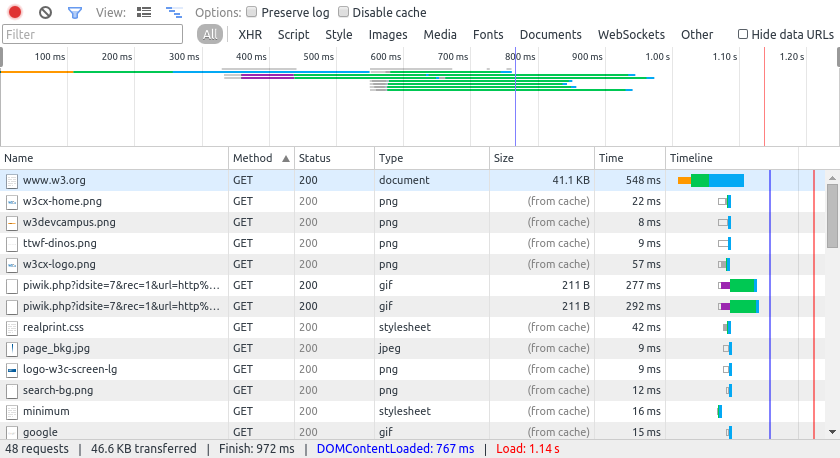
\includegraphics[width=\linewidth]{HTTP_Example}
	\caption{Google Developer Tools window showing HTTP Requests}	
\end{figure}

In the above example only the GET HTTP method is used, because the client only requests data from the server, without sending any data itself. If the client needs to send data to the server, such as form data, or a file, it would still initiate the connection (the server cannot make requests, only respond), using the POST method. While this approach is suitable for a passive, document-based web, where interaction is limited to jumping from document to document, the web has quickly evolved into an application-based model, where full UIs take place in the browser space, requiring data be constantly sent back and forth between client and server, in realtime. This project is one such application.\\

The only way to do this with standard HTTP is periodic polling, which entails large server and network loads. Some stopgap solutions exist to minimize this overhead, most relevant of which is the Comet web application model. Comet is based on the concept of long-polling: effectively ``hanging'' the server response until the requested data is available, and calling another request once the data is received. This approach  still causes increased server loads but allows some semblance of realtime data transmission. The possibility to use only one connection, as seen in the previous example was another improvement that became standard in HTTP 1.1. With the HTTP/2 Standard (published in May 2015), the server is allowed to effectively ``push'' data to clients by queuing up more responses than received requests. However, none of these modifications and hacks are a full solution to the problem, given that HTTP was never intended to be a realtime protocol.\\

That is why other technologies have taken over this new realm of interactivity, providing much more than the ``big, virtual documentation system in the sky'' envisioned by Berners-Lee more than 25 years ago. Some of them are key parts of this project, as the following sections describe. Still, HTTP remains the initiator for all these other technologies to function. As of today, any web page you open, no matter how complex the code served in javascript or flash or any other plugin still begins with a simple GET request and response.
\section{HTML}
\section{JavaScript}
\section{CSS}
\section{HTML5}
\section{WebSockets}
\section{The MEAN Stack}
\subsection{NodeJS}
\subsection{Express}
\subsection{MongoDB}
\subsection{AngularJS}
\section{Python}
\section{Development Environment \& Tools}
\subsection{Linux}
\subsection{Sublime Text}
\subsection{Git}
\subsection{\LaTeX}
\subsection{PM2}
\section{Hardware}
\subsection{Khepera III}
\subsection{Crazyflie 2}
\subsection{Raspberry Pi 2}
